
\chapter{The LHC Accelerator and the CMS Experiment}\label{ch:lhcandcms}
In the 1960s Peter Higgs \cite{peter_higgs}  and others \cite{other_1,other_2} put up the finishing touches on a theory combining three of the four fundamental forces and explainign how gauge bosons acquire mass. Nowadays this theory is known as the Standard Model (SM) of particles physics. It predicted the existence of several particles which were discovered in following decades. However, one particle was proving to be elusive, the so-called Higgs bosson. With this in mind the European Council for Nuclear Research (CERN) started plans to build an accelerator large enough and with the sufficient energy to prove the existance of the Higgs boson. Hence, the Large Hadron Collider (LHC) was born. 

\section{The LHC Accelerator}
The large hadron collider, shown in figure \ref{cern_fac}, is the biggest particle accelerator built by mankind to date. It has 27 km in circumference and is located in the French-Swiss border outside of Geneva, Switzerland \cite{lhc}. Using the previous installations as the large electron-positron collider the LHC can be operated in \pp mode or heavy ion mode. In \pp mode\footnote{Only \pp collision and considered in this document.}, the LHC accelerates two beams of protons in opposite directions until they collide at different points. In its initial physics run in 2011 and 2012, the LHC collided protons every 50 ns, at a center of mass energy of 7 Tera electron Volts (TeV), reached a peak luminosity of $ 7.7$ x $10^{33} cm^{-2} s^{-1}$\footnote{The LHC design luminosity is $10^{34} cm^{-2} s^{-1}$}, and delivered an integrated luminosity of $\approx 25 fb^{-1}$ to each of its two general purpose experiments, ATLAS and CMS. The analysis of this data yielded many physics results including the discovery of the Higgs boson published in 2013 \cite{atlas_higgs,cms_higgs}. During the following years the collider's luminosity was increase and its bunch crossing time reduced allowing for the Higgs boson properties to be measured. 

\begin{figure}[!t]
	\centering
	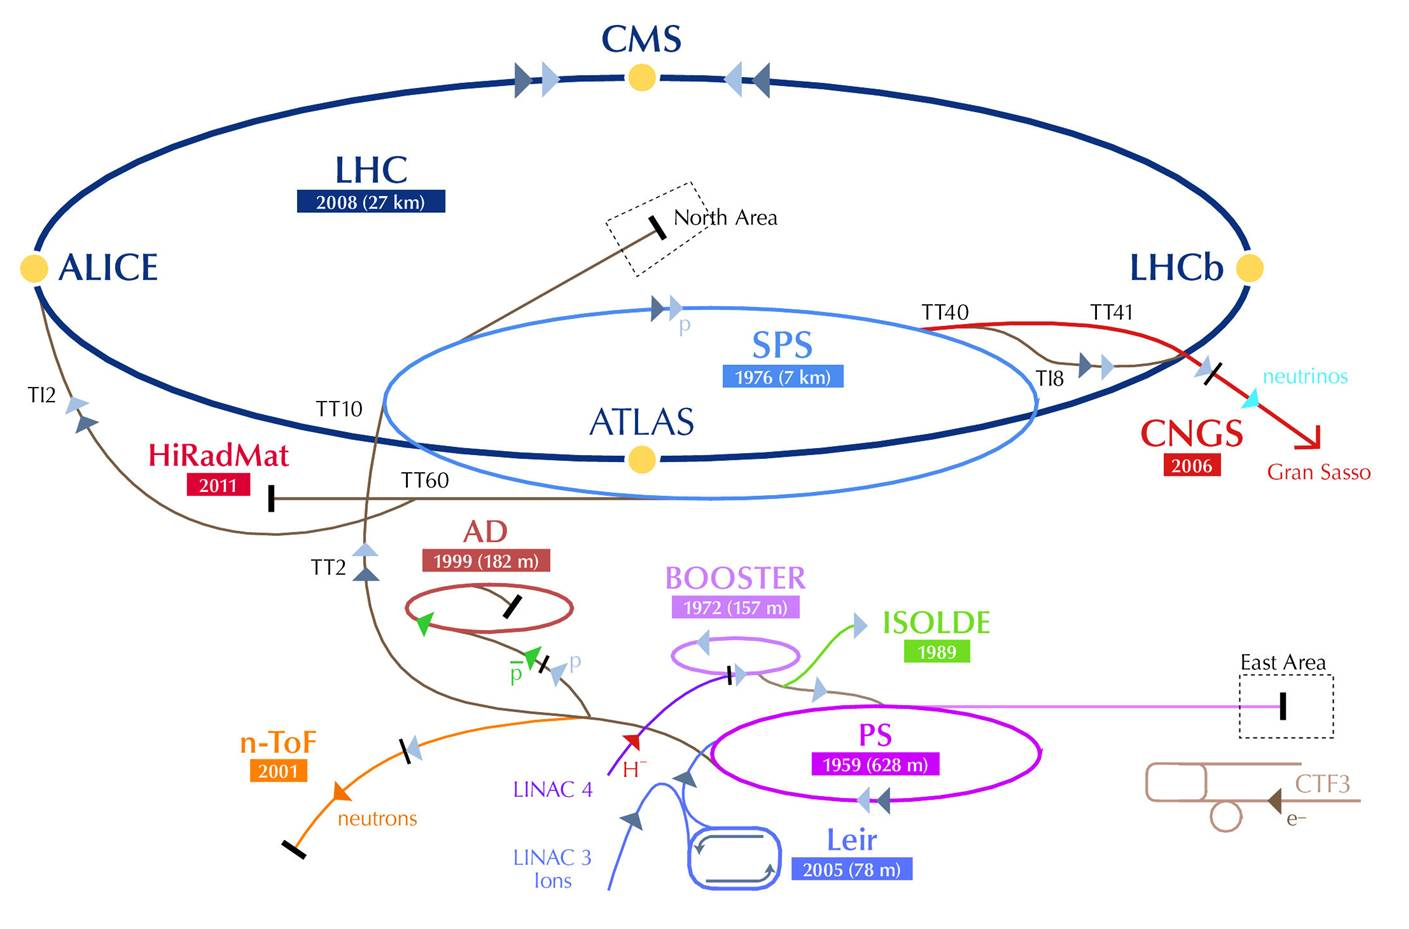
\includegraphics[width=0.7\textwidth]{/ch2/lhc_acce}
	\caption[The CERN acceleration \ital{facilities}]{The CERN acceleration \ital{facilities} showing the location of the four main experiment as well as the acceleration process[need ref].}
	\label{cern_fac}
\end{figure}

Four experiments were designed and built along the 27 km of the LHC ring. %to test different physics theories and search for new particles at the LHC.
Two of them, A Toroidal Large Aparatus (ATLAS)\cite{atlas} and the Compact Muon Solenoid (CMS)\cite{cms_doc} are large multipurpose experiments. The third experiment is LHCb \cite{lhcb}, which is specifically dedicated to study B-meson physics, the last experiment ALICE \cite{alice}, A Large Ion Collider Experiment, is dedicated to investigate heavy ion collisions.

%ls1 2013... energy to 13 tev\\
%ls2 2018... injecttor chsin improve
%\lipsum[1]
%The LHC, the biggest particle accelerator {\rojo{built}} by mankind to date, was built in the french-Swiss border outside of Geneva, Switzerland. A circular ring of 27 km built at the European Council for Nuclear Research (CERN) using the same tunnel . It   Tera electron Volts (TeV), making the center of mass energy 14 TeV. 
 



%It began operation in 2010 after two years solving issues that cause a false start in 2008. The LHC prove soon to be a success and in just two years of operations dele  



%The protons starts from a botle of hydrogen 

%With 27 km of circumference, the LHC is currently the most powerful circular acceler- ator in the world. It is installed in the same tunnel where the Large Electron-Positron (LEP) collider was located, taking advantage of the existing infrastructure. The LHC is part of the CERN’s accelerator complex composed of several successive accelerat- ing stages before the particles are injected into the LHC ring where they reach their maximum energy (see Figure 3.1).







%\begin{figure}[!h]
%	\centering
%	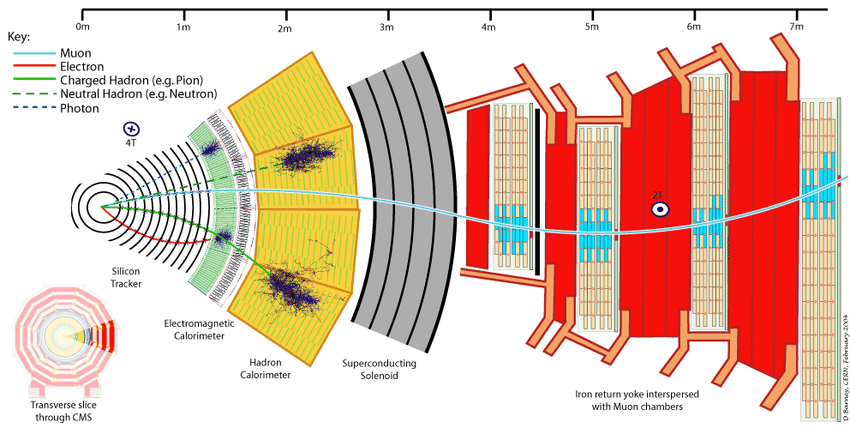
\includegraphics[width=0.7\textwidth]{ch2/cms_cross}
%	\caption[LHC dipoles]{LHC dipoles.}
%	\label{fig:cmscross}
%\end{figure}

\section{The CMS Experiment}
The compact muon soleinod, shown in figure \ref{cms_det} is one of the two multipurpose experiment at the LHC. The two main goals of the CMS experiment was to measure SM parameter with high precision as well as to test different physics theories beyond the standard model (BSM), i.e. SUSY, Dark matter and Dark energy, etc. The first goal has been achieve,    

\begin{figure}[!h]
	\centering
	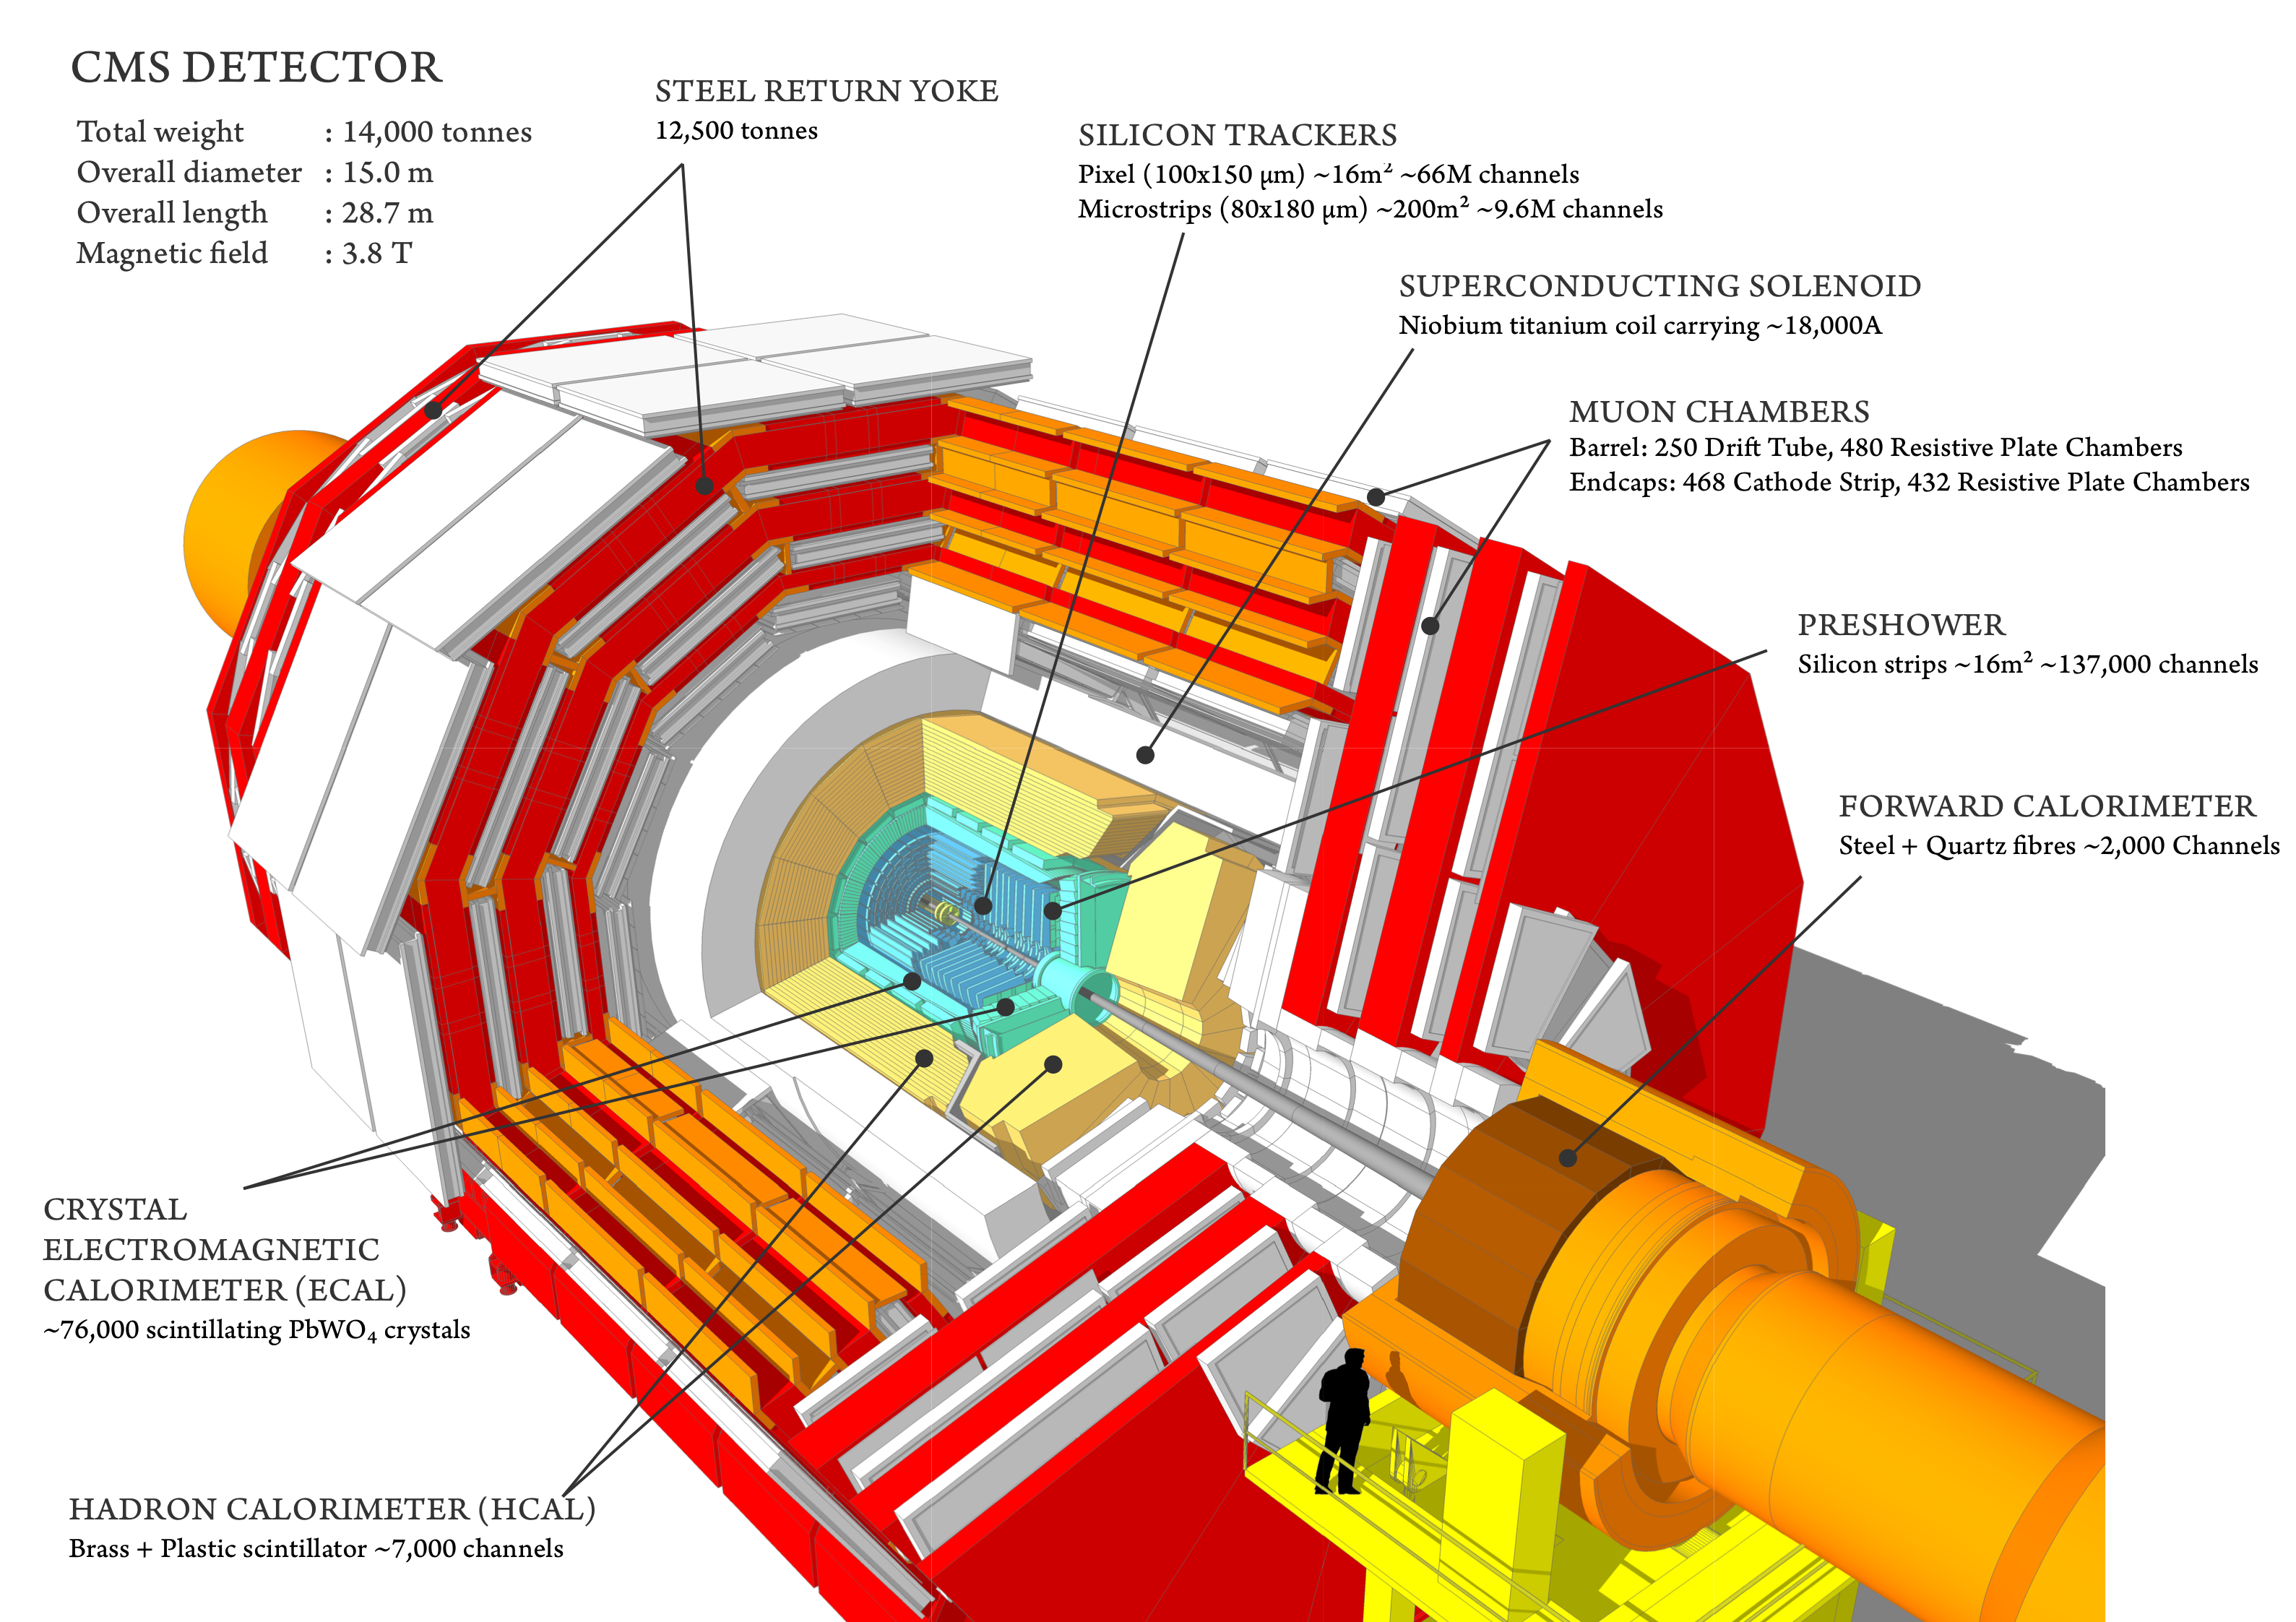
\includegraphics[width=0.7\textwidth]{ch2/cms_det2}
	\caption[CMS detector]{CMS detector \cite{cms_web}.}
	\label{cms_det}
\end{figure}

%https://cms.cern/news/first-measurement-lhc-run-2-pp-data-collected-2016-2017-and-2018
during its running years CMS has collected more than $ 160 fb^{-1}$ of data. This has yielded numerous phisics results luminosity a total of aspect To achieve its goal
\begin{figure}[!h]
	\centering
	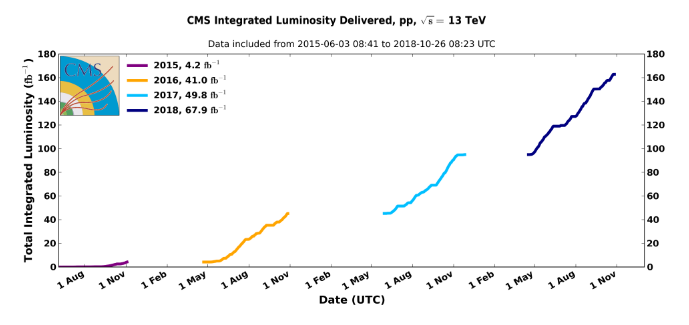
\includegraphics[width=0.7\textwidth]{ch2/cms_lumi}
	\caption[LHC luminosity]{Total integrated luminosity delivered by the LHC machine to the CMS experiment from 2015 to 2018 \cite{cms_lumi}}.
	\label{lumi2016}
\end{figure}




%images: 
%run276282->An event where two Z candidates are produced and each decay into two muons, each given by the red lines. This event has 27 reconstructed vertices. (CMS SketchUp model by Tai Sakuma) (Image: CERN)
%fig1 gammagamma 


CMS is one of two general purpose experiments at the LHC and it is located at Point 5 as
shown in Fig. 1.2. It is designed to take data using both proton-proton and ion-ion collisions.
The main physics goals are the search for the SM Higgs boson and physics beyond the SM,
heavy quarks, and heavy ion physics.
CMS has to fulfill several requirements [15]:


Good muon identification and momentum resolution over a wide range of momenta in
the pseudorapidity 3 region η < 2.5, good dimuon mass resolution (≈ 1% at 100 GeV/c 2 ),
and the ability to determine unambiguously the charge of muons with p < 1 TeV/c.
• Good charged particle momentum resolution and reconstruction efficiency in the inner
tracker. Efficient triggering and offline tagging of τ ’s and b-jets, requiring pixel detectors
close to the interaction region.
• Good electromagnetic energy resolution, good diphoton and dielectron mass resolution
(≈ 1% at 100 GeV/c 2 ), wide geometric coverage (η < 2.5), measurement of the direction
of photons and/or correct localization of the primary interaction vertex, π 0 rejection and
efficient photon and lepton isolation at high luminosities.
• Good transverse missing energy E T miss and dijet mass resolution, requiring hadron calorime-
ters with a large hermetic geometric coverage (η < 5) and with fine lateral segmentation.
The requirements above led to the detector design shown in Fig. 1.3. Ideally, the detector
shape would be spherical for best hermeticity but this is almost impossible technically. A
cylindrical shape therefore is chosen to achieve very good geometrical coverage and include a
magnetic solenoid for particle momentum measurements.

CMS comprises several sub detectors (see Fig. 1.3). An assembled part of the CMS exper-
iment in SX5 underground is shown in Fig. 1.4. The sub detectors from the innermost to
outermost are
• the inner tracker (silicon strips and pixels)
• the electromagnetic calorimeter
3
6
• the hadronic calorimeter and


The origin of the CMS coordinate system is at the interaction point, the y-axis pointing
vertically upward, and the x-axis pointing radially inward towards the center of the LHC
ring. The z-axis points along one of the beam direction (towards the Jura mountains). The
azimuthal angle φ is measured from the x-axis in the x-y plane. The polar angle θ is measured
from the z-axis. These coordinates will also be used later in this thesis.


1.3.1 Magnet
As mentioned before, CMS requires a high performance of the muon system and a momentum
resolution of 10% at p = 1 TeV/c. Therefore a large magnet is chosen for CMS [16], composed
of a superconducting solenoid and a magnet yoke. The solenoid is 13 m long and has an
inner diameter of 6 m. It contains the tracker and calorimeters. The magnetic field inside
the solenoid is 4 T while in the yoke it is 2 T. The bending direction within the solenoid is
opposite to the one in the magnet yoke, as shown in Fig. 1.5. This provides a longer path for
the energetic muons, increasing the precision of muon momentum measurements.


1.3.2 Inner tracking system
The expected charged particle flux as a function of the distance to the interaction point
determined the design of the inner tracker system. At a distance of 4 cm a flux of up to 100
MHz/cm 2 is expected. The innermost part of the tracker will be exposed to very high radiation
doses, with time causing severe radiation damage to the tracker material. The radiation dose is proportional to 1/r 2 , where r is the radius of the tracker layer. The expected radiation dose
and hadron fluence in radial layers of the CMS tracker are shown in Table 1.2 for different
radii. It is worth mentioning that a few Grays of dose is lethal for human. One of the main
challenges is to operate the tracker in such a harsh environment for an expected lifetime of 10
years at the full LHC luminosity 10 34 cm 2 s −1 . The radiation hardness, granularity and speed
requirements favored devices based on silicon technology.



\begin{figure}[!h]
	\centering
	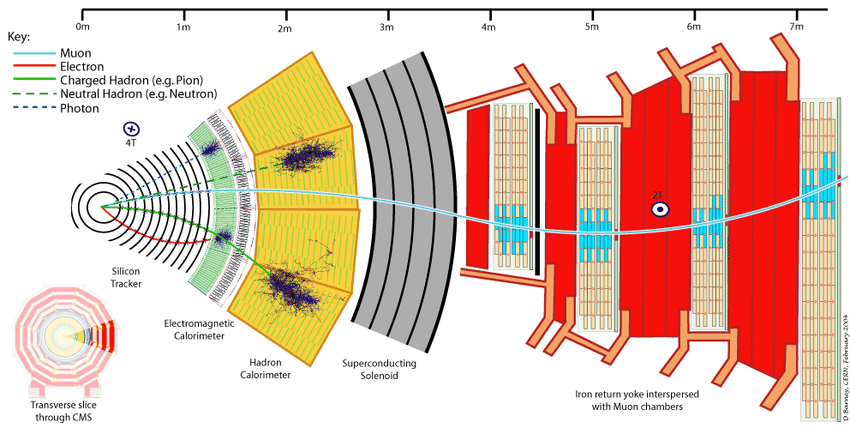
\includegraphics[width=0.7\textwidth]{ch2/cms_cross}
	\caption[CMS cross sectional view]{CMS cross sectional view.}
	\label{cmscross}
\end{figure}

\begin{figure}[h!]
	\centering
	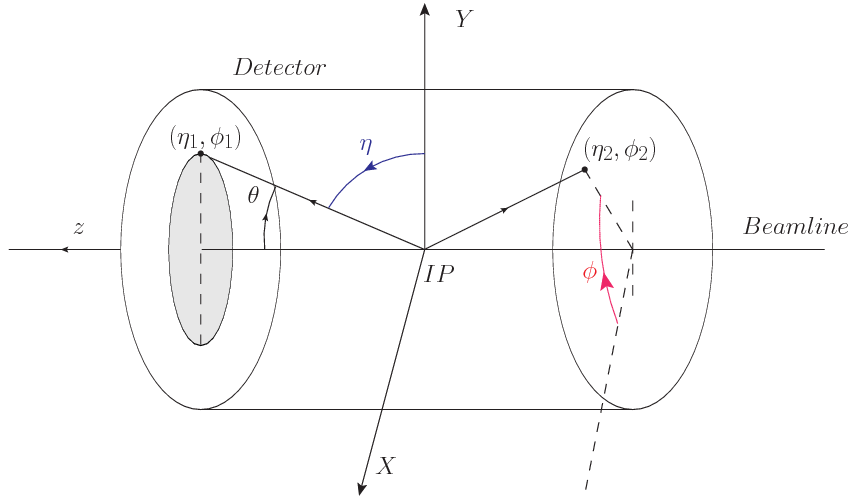
\includegraphics[scale=0.4]{ch2/coord}
	\caption[CMS detector coordinate system]{CMS detector coordinate system \cite{and_the}.}
	\label{fig:coord}
\end{figure}

Describe from the outside the CMS experiment subdetector are: the muon chambers, the hadronic calorimeter, the Electromagnetic calorimeter, the superconducting solenoid, and the tracker detector which is composed of the silicon strips and the pixel detector.

\subsection{The Muon Chambers}
Muons have a relatively long lifetime of 2.2 μs. They interact weakly with matter and are
not stopped by the calorimeters where they deposit some of their energy. The CMS muon
detectors therefore are the outermost sensitive devices in the experiment [21]. The muon
detectors are divided into a barrel and two end cap regions. The system utilizes three different
technologies: drift tubes (DT) in the barrel region, cathode strip chambers (CSC) in the end-
cap region and resistive plate chambers (RPC) in both barrel and end-cap regions. The RPCs
provide a trigger signal while DT and CSC detectors can reconstruct the muon trajectory and
momentum. The muon system covers the region |η| < 2.4. The muon system is important for
muon identification. For transverse momenta below 200 GeV the muon identification relies on
the inner tracker.
%\begin{figure}[!h]
%	\centering
  %
\includegraphics[width=0.7\textwidth]{../images/ch2/9}
  %\caption[The Muon Chambers]{The Muon Chambers.}\label{fig:cms_layout}
%\end{figure}
\subsection{The Hadronic Calorimeter}

Similar to the ECAL the aim of the hadronic calorimeter (HCAL) is to measure the energy
and the direction of strongly interacting particles and jets as well as missing transverse energy.
The CMS HCAL [20] surrounds the ECAL. It has a sandwich structure of brass absorbers and
plastic scintillators. The reason for choosing these materials is that they have smaller radiation
lengths which minimize multiple scattering for traversing muons. The hadron barrel and end
caps cover the range |η| < 3 with higher granularity. There are additional scintillators installed
inside the muon barrel layer and steel-quartz fibers in the very forward region providing overall
pseudorapidity coverage of |η| < 5.
%\begin{figure}[!h]
 % \centering
  %
\includegraphics[width=0.7\textwidth]{../images/ch2/8}
%  \caption[The Hadronic Calorimeter]{The Hadronic Calorimeter.}\label{fig:cms_layout}
%\end{figure}

%\begin{figure}[!h]
%	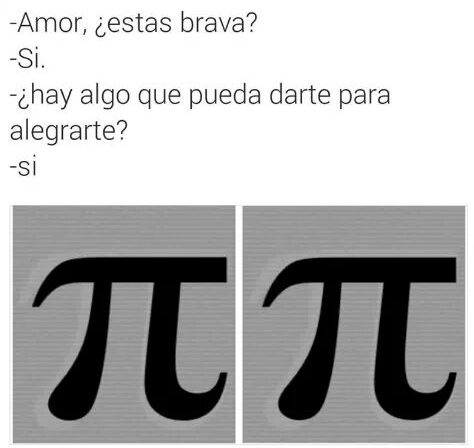
\includegraphics[width=0.7\textwidth]{ch2/8}
%  \caption[The Hadronic Calorimeter]{The Hadronic Calorimeter.}\label{fig:cms_layout}
%\end{figure}
\subsection{The Electromagnetic Calorimeter}
An electromagnetic calorimeter (ECAL) is used to measure the energy and direction of elec-
trons, photons, and jets. Measurements with very high precision are required. The CMS ECAL
is made of lead-tungstate (PbWO 4 ) crystals. The high density of the crystals (8.2 g/cm 3 ) leads to a short radiation length and narrow showers, which allow for a compact calorimeter inside
the solenoid that is fast, has fine granularity, and is radiation resistant [19]. The ECAL pseudo-
rapidity coverage is |η| < 3. Particle induced scintillation light is detected by silicon avalanche
photodiodes (APDs) in the barrel region and vacuum phototriodes (VPTs) in the end cap
region.
%\begin{figure}[!h]
%	
\includegraphics[width=0.7\textwidth]{ch2/7}
%	\caption[The Electromagnetic Calorimeter]{ The Electromagnetic Calorimeter.}\label{fig:cms_layout}
%\end{figure}

\subsection{The Tracker Detector}

%\begin{figure}[!h]
 % \centering
  %
\includegraphics[width=0.7\textwidth]{ch2/3}
  %\caption[CMS Tracking system.]{CMS Tracking system.}\label{fig:cms_layout}
%\end{figure}

\subsubsection{Silicon Strips}

%\begin{figure}[!h]
 % \centering
  %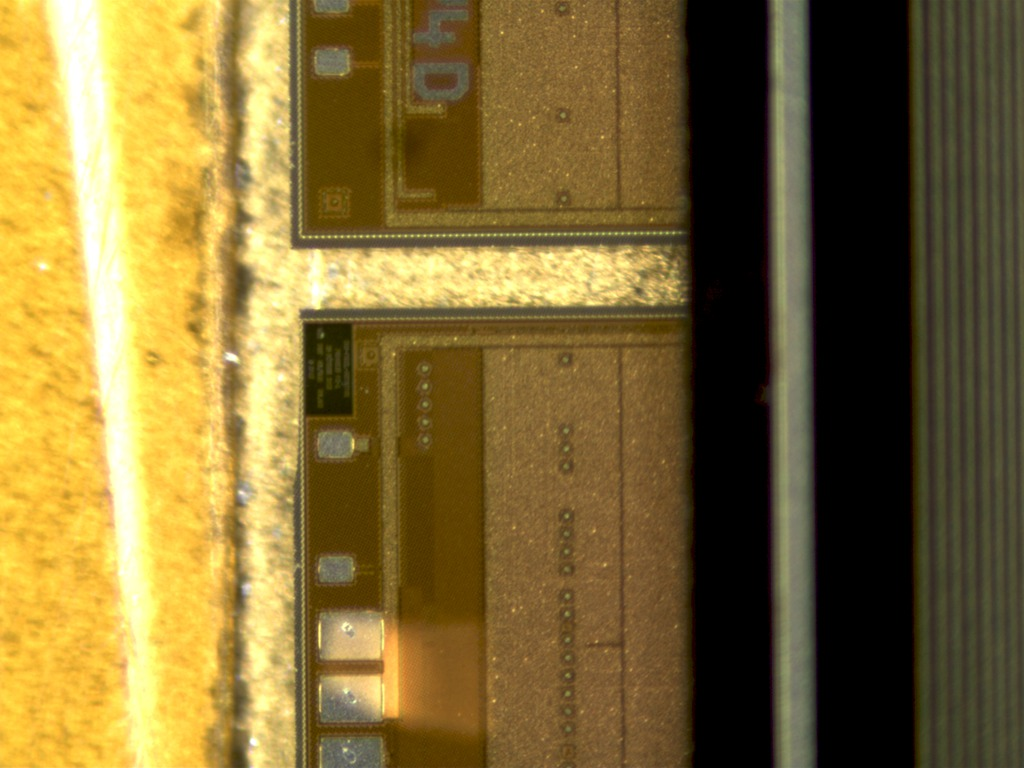
\includegraphics[width=0.7\textwidth]{ch2/6}
 % \caption[silicon strips detector]{silicon strips detecto.}\label{fig:cms_layout}
%\end{figure}

\subsubsection{Pixel Detector}
Being the innermost detector in CMS, the pixel detector works in a high radiation environment but, due to its excellent design and construction, it performed well during the initial CMS run. It provided two or more hits per track, allowing secondary vertex identification of long-lived objects. The pixel detector is composed of two parts, the barrel (BPix) and a disk at each end, denominated Forward pixel detector (FPix), as showing in figure \ref{pixeldetector}. The BPix is made of three layers located at 4.3 cm, 7.2 cm, and 11.0 cm from the interaction point respectively. The FPix has two layers, one at 34.5 cm and the other at 46.5 from the interaction point. This thesis will focus on the FPix, the part of the detector where UNL has made major contributions in the last {\rojo{two}} three decades.  

\begin{figure}[!h]
	\centering
	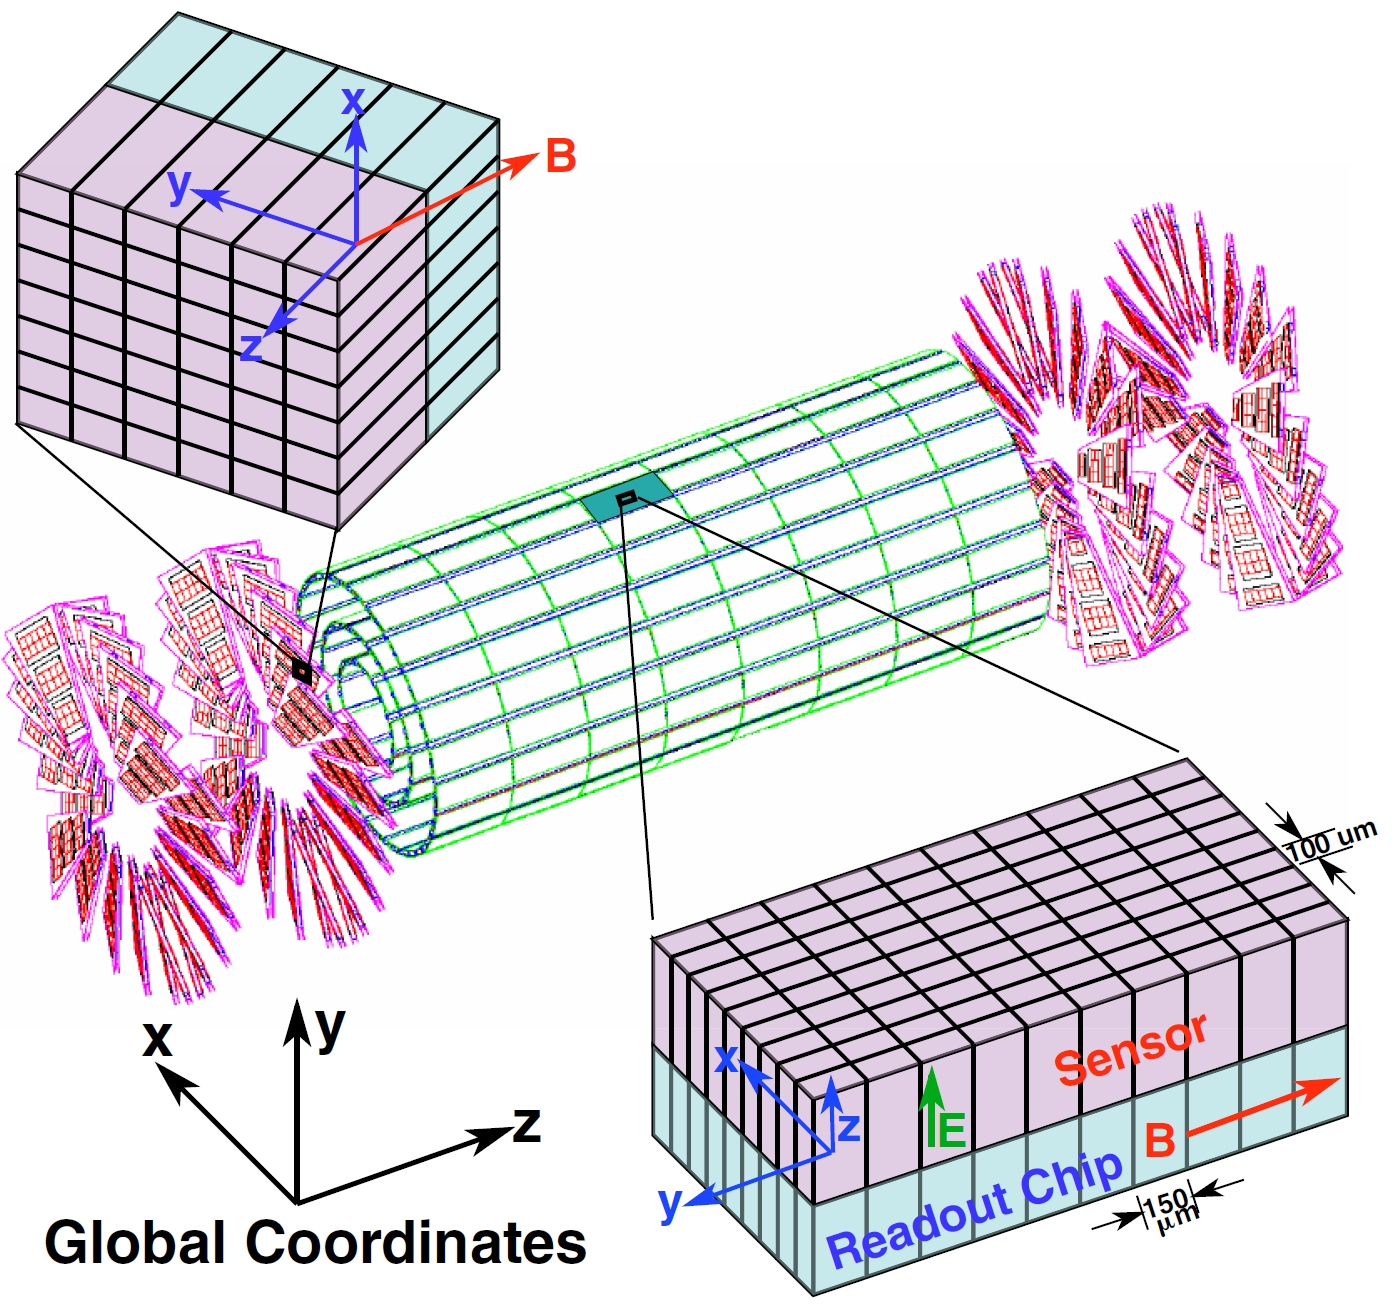
\includegraphics[width=0.7\textwidth]{ch2/pixel_detector}
	\caption[Pixel detector]{Pixel detector.}
	\label{pixeldetector}
\end{figure}

  

The original FPix, also known as phase 0, was populated by 672 modules of 100 by 100 $\mu m$ 
\subsubsection{The trigger}
The CMS trigger system has a two step decision system after which events will be recorded.
The first trigger level, Level 1, decreases the event rate from 40 MHz to 100 kHz. The Level 1
is implemented in hardware and its decision takes 3.2 μs. This level requires information from
the calorimeters and the muon detectors. The second level is known as High Level Trigger
(HLT). The HLT is implemented in software. It uses the data from all CMS subdetectors. The
event rate is reduced to 150 Hz at this level.



